% =========================================================
%  Springer LNCS Camera-Ready Manuscript — CVIP 2026
%  Paper 544: Federated Learning for Massive MIMO
%  Channel Estimation Under IID and Non-IID Client Data
% =========================================================
\documentclass[runningheads]{llncs}

% --- Required packages (minimal, LNCS-compatible) -------
\usepackage{cite}
\usepackage{amsmath,amssymb}
\usepackage{graphicx}
\usepackage{booktabs}
\usepackage{multirow}
\usepackage{array}
\usepackage{url}
% --------------------------------------------------------
% NOTE: fancyhdr removed — Springer LNCS controls headers
%       float [H] replaced with [htbp] throughout
%       linespread and manual spacing hacks removed
% --------------------------------------------------------

\title{Federated Learning for Massive MIMO Channel
  Estimation Under IID and Non-IID Client Data}

% Author block: names, ORCID stubs, affiliation, email
\author{
  Jagadeesh Kakarla\inst{1}\orcidID{0000-0000-0000-0000} \and
  Koppaku Krishna Chaitanya\inst{1}\orcidID{0000-0000-0000-0001} \and
  Kappala Akshay\inst{1}\orcidID{0000-0000-0000-0002} \and
  Dammala Basava Sri Ram\inst{1}\orcidID{0000-0000-0000-0003} \and
  Yaparla Sainatha Reddy\inst{1}\orcidID{0000-0000-0000-0004}
}

\authorrunning{J.~Kakarla et al.}

\institute{
  Indian Institute of Information Technology, Design and Manufacturing,
  Kancheepuram, India\\
  \email{jagadeeshk@iiitdm.ac.in}\textsuperscript{\,\dagger}
}
% \textsuperscript{\dagger} marks the corresponding author

\begin{document}

\maketitle

% ---------------------------------------------------------
\begin{abstract}
  Accurate channel state information (CSI) acquisition is fundamental to
  realising the spatial-multiplexing gains of Massive MIMO systems.
  Conventional deep-learning approaches train models on centrally
  aggregated pilots, incurring substantial uplink overhead and raising
  serious privacy concerns.  We present a reproducible federated-learning
  (FL) benchmark for massive MIMO channel estimation that eliminates the
  need for raw data transfer.  Lightweight convolutional (CNN) and
  encoder-decoder (ResUNet) architectures are trained with FedAvg and
  FedProx under both identically distributed (IID) and heterogeneous
  (Non-IID) client partitions, systematically constructed to mimic
  geographically dispersed user equipment.  Our benchmark demonstrates
  that FedAvg under IID data marginally surpasses the centralized
  baseline ($-20.04$\,dB vs.\ $-19.62$\,dB NMSE), while Non-IID
  heterogeneity introduces a statistically significant degradation of up
  to $0.57$\,dB.  FedProx stabilises convergence trajectories but does
  not consistently improve mean NMSE in the tested regime, a finding we
  attribute to proximal over-regularisation at limited local epochs.
  All experimental protocols, data splits, and trained weights are
  publicly released to support reproducibility.
\keywords{Federated learning \and massive MIMO \and channel estimation
  \and non-IID data \and FedAvg \and FedProx \and reproducibility}
\end{abstract}

% ---------------------------------------------------------
\section{Introduction}
\label{sec:intro}

The evolution of wireless infrastructure toward 5G and beyond places
stringent requirements on spectral efficiency, massive device
connectivity, and ultra-reliable low-latency communication.  Massive
Multiple-Input Multiple-Output (Massive MIMO) systems, which deploy
hundreds of antennas at the base station (BS), address these demands
through aggressive spatial multiplexing and directional beamforming.
However, the practical gains of Massive MIMO are contingent on accurate
knowledge of the Channel State Information (CSI) at the receiver.

Classical pilot-based estimators---including Least Squares (LS) and
Minimum Mean Square Error (MMSE)---remain the established benchmarks.
The LS estimator is computationally inexpensive but is highly sensitive
to additive noise.  The full-covariance MMSE (Wiener filter) achieves
the optimal linear bound, yet requires an explicit channel covariance
matrix $R_{HH}$ and an $O(d^3)$ matrix inversion for $d = N_t N_s$,
which is prohibitive for the large array dimensions of Massive MIMO.

Deep learning (DL) has emerged as a powerful alternative, with
convolutional and encoder-decoder models demonstrating strong channel
estimation accuracy without explicitly computing channel
statistics~\cite{wen2018deep,he2018deep,ye2018power,soltani2019deep}.
However, conventional DL training assumes centralised data collection:
user equipment (UE) must transmit high-dimensional raw CSI measurements
to a central server, creating prohibitive uplink overhead and exposing
sensitive location-correlated information.

Federated Learning (FL) resolves this tension by enabling a global
model to be trained through local gradient updates that never leave each
client device~\cite{mcmahan2017fedavg,kairouz2021survey}.  The server
aggregates only model parameters, not raw channel data.  Nevertheless,
the performance of FL is sensitive to statistical heterogeneity across
clients: in real wireless deployments, UEs at different geographical
locations experience distinct SNR regimes, propagation environments, and
scattering conditions, naturally producing Non-IID local
datasets~\cite{ghosh2019robust}.  Understanding and quantifying this
heterogeneity penalty is essential before deploying FL-based channel
estimators in practice.

This work makes the following contributions:
\begin{enumerate}
  \item A \textbf{systematic, reproducible benchmark} for FL-based
        Massive MIMO channel estimation using the DeepMIMO O1\_60
        ray-tracing scenario.
  \item A \textbf{structured IID/Non-IID protocol} whose Non-IID
        partitions explicitly mimic the SNR diversity experienced by
        geographically separated users.
  \item \textbf{Dual-architecture validation} (CNN and ResUNet) with
        FedAvg and FedProx, enabling the assessment of whether
        heterogeneity findings generalise across model capacity.
  \item \textbf{Communication and complexity analysis} quantifying
        uplink payload and FLOPs per inference for practical deployment
        planning.
  \item \textbf{Statistical validation} using Welch's $t$-tests to
        confirm that observed performance gaps are not artefacts of
        random seed variation.
\end{enumerate}

% ---------------------------------------------------------
\section{Related Work}
\label{sec:related}

The closest related work is that of Elbir and Coleri~\cite{elbir2021flchannel},
who propose an FL framework for channel estimation in both conventional
and RIS-assisted Massive MIMO and demonstrate an uplink communication
reduction factor of approximately $16\times$ relative to centralised
learning.  Our work shares the same motivation of minimising data
transfer overhead via FL, but differs in three important respects:
(i)~we explicitly quantify the IID-to-Non-IID degradation through a
structured partitioning protocol; (ii)~we provide dual-architecture
validation across CNN and ResUNet models; and (iii)~we release fully
reproducible code, data splits, and weights.
Table~\ref{tab:alignment_ec} summarises the alignment with
Elbir--Coleri~\cite{elbir2021flchannel}.

The foundational FL algorithms are FedAvg~\cite{mcmahan2017fedavg} and
FedProx~\cite{li2020fedprox}.  A comprehensive treatment of open
problems in federated learning, including data heterogeneity, appears
in~\cite{kairouz2021survey}, while~\cite{ghosh2019robust} analyses
robustness to heterogeneous environments.  For background on machine
learning in RIS-assisted wireless systems, we refer the reader to the
survey by Faisal and Choi~\cite{faisal2022rismlsurvey}.

\begin{table}[htbp]
\caption{Alignment of the proposed work with Elbir--Coleri~\cite{elbir2021flchannel}.}
\label{tab:alignment_ec}
\centering
\begin{tabular}{p{0.24\linewidth}p{0.33\linewidth}p{0.30\linewidth}}
\toprule
Aspect & Elbir--Coleri (TWC) & Proposed Work \\
\midrule
Primary objective  & Reduce CL uplink overhead via FL
                   & Same objective with structured heterogeneity analysis \\
Task               & FL channel estimation
                   & FL channel estimation \\
Scenario           & Conventional + RIS-assisted Massive MIMO
                   & DeepMIMO O1\_60 Massive MIMO \\
Model family       & CNN-based ChannelNet
                   & CNN (primary) + ResUNet (validation) \\
Learning modes     & CL vs.\ FL
                   & CL vs.\ FL (FedAvg / FedProx) \\
Heterogeneity      & Non-IID challenge discussed qualitatively
                   & Explicit IID/Non-IID protocol; quantified deltas \\
Statistical tests  & Not reported
                   & Welch's $t$-test for all key comparisons \\
Reproducibility    & Partial
                   & Full (code, splits, and weights released) \\
\bottomrule
\end{tabular}
\end{table}

% ---------------------------------------------------------
\section{System Model and Problem Formulation}
\label{sec:system}

\begin{figure}[htbp]
\centering
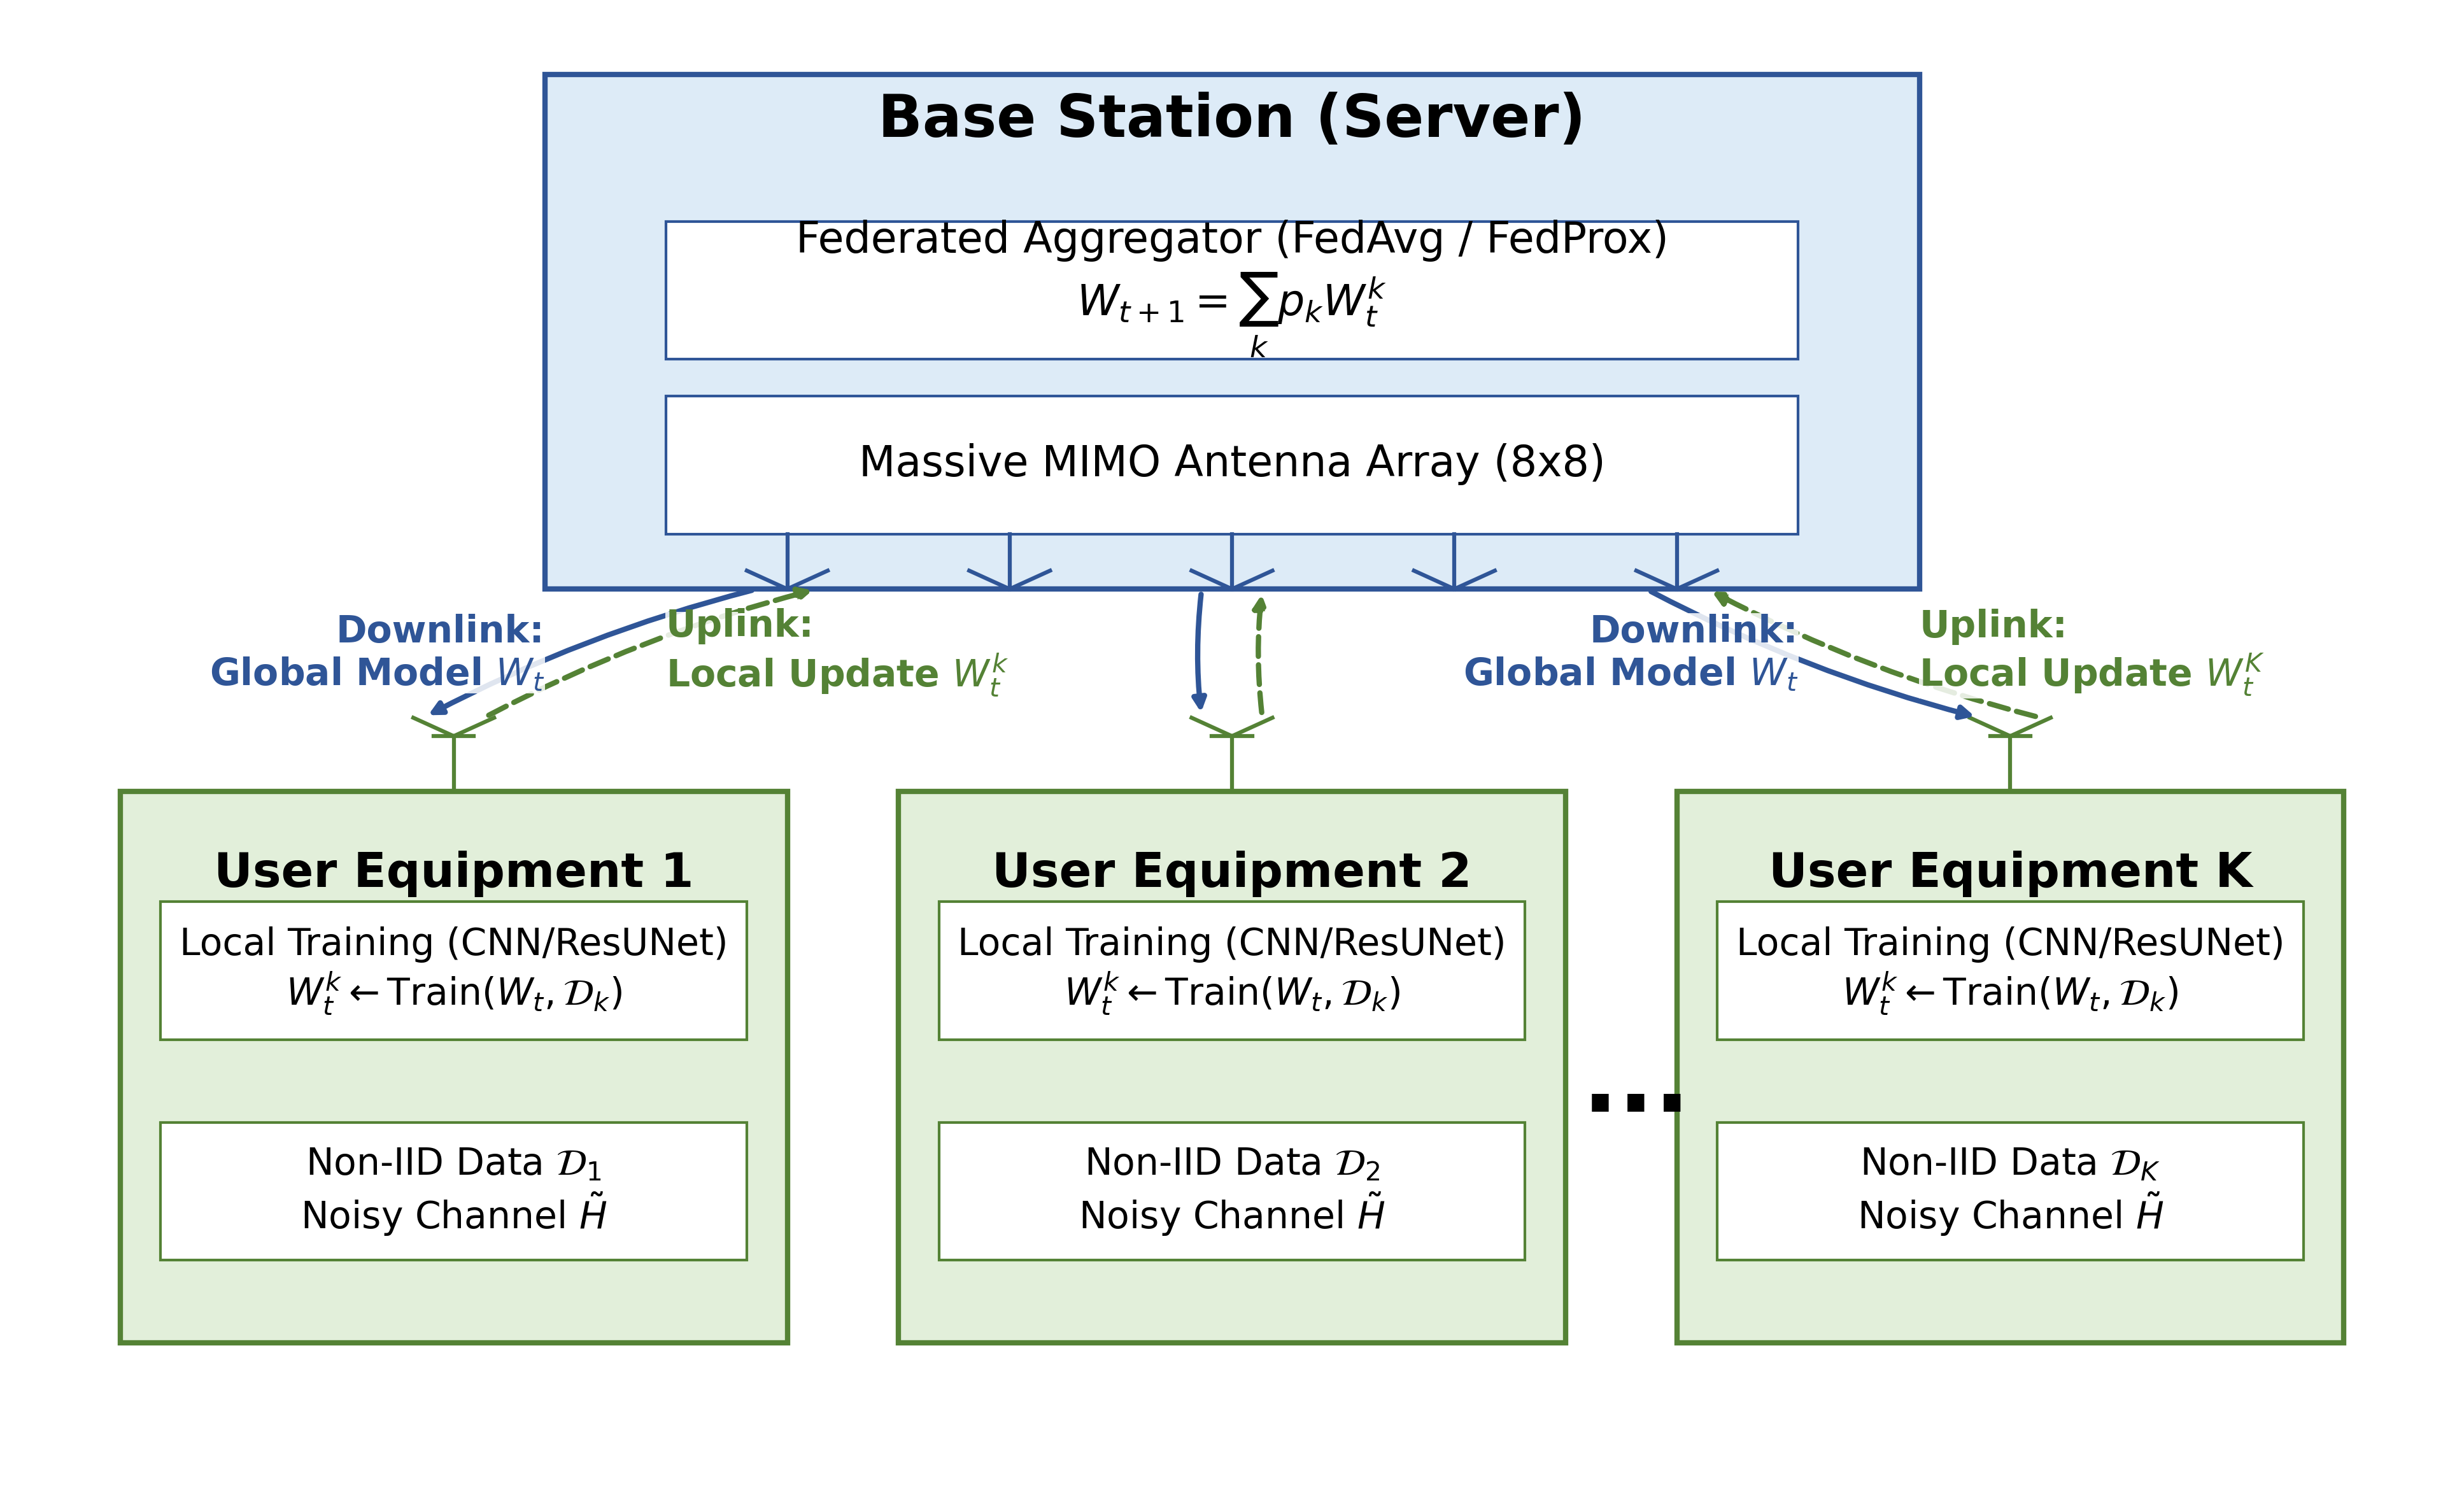
\includegraphics[width=\columnwidth]{figures/system_architecture_diagram.png}
\caption{End-to-end federated learning pipeline for Massive MIMO
  channel estimation.  User equipment (UE) devices perform local CSI
  model updates on private pilot observations; the base station (BS)
  aggregates model parameters without accessing raw channel data,
  preserving user privacy.}
\label{fig:system_model}
\end{figure}

Fig.~\ref{fig:system_model} illustrates the proposed federated pipeline.
The BS deploys $N_t$ antennas and serves single-antenna UEs over $N_s$
OFDM subcarriers.  Let $H \in \mathbb{C}^{N_t \times N_s}$ denote the
clean channel response and $\tilde{H}$ the pilot-contaminated noisy
observation obtained after standard OFDM pilot extraction.  The
estimator $f_\theta : \tilde{H} \mapsto \hat{H}$ is parameterised by
$\theta$ and trained to minimise the mean squared error.  Performance is
measured by Normalised Mean Squared Error (NMSE) in decibels:
\begin{equation}
  \mathrm{NMSE}_{\mathrm{dB}}
    = 10\log_{10}\!\left(\frac{\|H - \hat{H}\|_2^2}{\|H\|_2^2}\right).
  \label{eq:nmse}
\end{equation}

In the centralised (CL) baseline, all training samples are collected at
the BS.  In FL, client $k$ trains locally on its private dataset
$\mathcal{D}_k$ and transmits parameter updates to the BS.  FedAvg
aggregates these updates as a weighted average:
\begin{equation}
  \theta^{t+1} = \sum_{k=1}^{K} \frac{n_k}{\sum_j n_j}\,\theta_k^t,
  \label{eq:fedavg}
\end{equation}
where $n_k = |\mathcal{D}_k|$.  FedProx~\cite{li2020fedprox} augments
each client's local objective with a proximal term to limit divergence
from the global model:
\begin{equation}
  \min_{\theta_k} \; F_k(\theta_k) + \frac{\mu}{2}\|\theta_k - \theta^t\|_2^2,
  \label{eq:fedprox}
\end{equation}
where $\mu > 0$ controls the regularisation strength.

% ---------------------------------------------------------
\section{Proposed Methodology}
\label{sec:method}

The end-to-end pipeline comprises six stages:
(i)~channel generation via DeepMIMO ray-tracing,
(ii)~AWGN noise injection at multiple SNR levels with sample-wise power
normalisation,
(iii)~global normalisation and 80/20 train--test splitting per SNR,
(iv)~client data partitioning under IID and Non-IID protocols,
(v)~federated model training with FedAvg and FedProx,
and (vi)~performance evaluation on a held-out test set using
Eq.~\eqref{eq:nmse}.

\subsection{Dataset Construction}
\label{ssec:dataset}

The dataset is derived from the DeepMIMO O1\_60 outdoor ray-tracing
scenario~\cite{alkhateeb2019deepmimo}.  We select $6{,}000$ users from
base-station BS-0, configure an $8 \times 8$ BS antenna array ($N_t =
64$), a $1 \times 1$ UE array, and $N_s = 64$ OFDM subcarriers.
Circularly-symmetric complex Gaussian (AWGN) noise is added at
SNR~$\in \{0, 5, 10, 15, 20\}$\,dB using a fixed random seed (42) for
reproducibility.  Real and imaginary components are stacked to form a
two-channel real-valued representation suitable for standard
convolutional processing.  Training and test sets are formed by globally
shuffling the samples and applying an 80/20 split independently at each
SNR level.

\subsection{Deep Learning Models}
\label{ssec:models}

\textbf{CNN (Primary Benchmark).}
The CNN adopts a residual correction strategy: rather than mapping the
noisy input $\tilde{H}$ directly to $\hat{H}$, the network learns the
correction residual $\Delta H = H - \tilde{H}$, so that
$\hat{H} = \tilde{H} + f_\theta(\tilde{H})$.  The architecture consists
of (i)~a feature extraction head comprising a Conv2D layer (2$\to$32
channels, $3\times 3$ kernel) with batch normalisation and ReLU
activation; (ii)~a single residual block (two 32-channel Conv2D layers
with a skip connection); and (iii)~a reconstruction tail (Conv2D,
32$\to$2 channels).  The total parameter count is $19{,}778$, making the
model well-suited for resource-constrained client devices.

\textbf{ResUNet (Cross-Architecture Validation).}
To assess whether the heterogeneity findings generalise beyond
lightweight models, we additionally train a ResUNet encoder-decoder
($763{,}234$ parameters, 15 layers).  The encoder comprises three
sequential convolutional blocks that halve spatial dimensions while
doubling channel depth (2$\to$128 channels); a residual bottleneck
preserves gradient flow; and the decoder upsamples via transposed
convolutions with skip connections that concatenate high-resolution
encoder features to recover fine spatial detail.

\subsection{IID and Non-IID Client Partitioning}
\label{ssec:partition}

\textbf{IID.} The full training dataset is globally shuffled and divided
uniformly into $K = 5$ client subsets of equal size.  Each client thus
receives a representative cross-section of the joint SNR distribution.

\textbf{Non-IID.} Real wireless deployments produce heterogeneous client
datasets because geographically separated UEs experience statistically
distinct propagation environments.  Users in dense urban areas encounter
rich scattering with high received SNR, while those at the cell edge or
in obstructed regions operate at low SNR with sparse multipath.  This
geographical diversity naturally produces datasets whose empirical
channel-power distributions differ substantially across devices.

To reproduce this effect in a controlled and reproducible manner, we
construct heterogeneous client datasets using a norm-based grouping
strategy.  Samples are sorted by their Frobenius norm $\|H\|_F$,
which serves as a proxy for received channel power.  Each client
$k$ receives a dataset composed of two complementary segments:
\begin{equation}
  \mathcal{D}_k = \mathcal{D}_k^u \cup \mathcal{D}_k^s,
  \qquad
  \rho = \frac{|\mathcal{D}_k^u|}{|\mathcal{D}_k|},
  \label{eq:noniid}
\end{equation}
where $\mathcal{D}_k^u$ is a \emph{unique} segment drawn from a
norm-sorted pool rotated by client index (so that each client
concentrates on a different power regime), and $\mathcal{D}_k^s$ is a
\emph{shared} global segment common to all clients.  The ratio
$\rho = 0.6$ is used for ResUNet experiments, meaning each client's
dataset is 60\% client-specific (high heterogeneity) and 40\% shared
(representing common propagation features seen by all users).
Norm-based grouping is preferred over random label-skew schemes because
it directly reflects the physical mechanism driving heterogeneity in
wireless channels: geographical SNR variation.  For CNN experiments,
heterogeneity is induced by rotating the source SNR pool across clients
via dedicated split scripts, producing equivalent structured skew.

% ---------------------------------------------------------
\section{Experimental Setup}
\label{sec:setup}

\subsection{Primary CNN Benchmark}

All primary experiments use $10$\,dB SNR.  The sweep covers:
\begin{itemize}
  \item \textbf{Centralised CNN:} 3 random seeds.
  \item \textbf{FedAvg-IID:} $R \in \{10, 20, 30, 50\}$ global rounds,
        $E \in \{1, 2, 3, 5\}$ local epochs, 3 seeds
        ($48$ total configurations).
  \item \textbf{FedAvg-Non-IID:} same $R$, $E$, 3 seeds ($48$ runs).
  \item \textbf{FedProx-Non-IID:} same $R$, $E$,
        $\mu \in \{0.001, 0.005, 0.01\}$, 3 seeds ($144$ runs).
\end{itemize}

\subsection{ResUNet Add-On Validation}

A 20-run protocol verifies cross-architecture consistency:
\begin{itemize}
  \item Centralised ResUNet: 5 seeds.
  \item FedAvg-IID: 5 seeds.
  \item FedAvg-Non-IID ($\rho = 0.6$): 5 seeds.
  \item FedProx-Non-IID ($\mu = 0.001$): 5 seeds.
\end{itemize}

\subsection{Classical Baselines}

Three classical estimators are evaluated at $10$\,dB to contextualise
the deep learning results:

\textbf{LS.} The least-squares estimator $\hat{H}_\mathrm{LS} =
\tilde{H}$ applies no noise suppression and therefore serves as the
lower performance bound.

\textbf{Scalar LMMSE.} A train-calibrated scalar shrinkage estimator:
\begin{equation}
  \hat{H}_\mathrm{scalar}
    = \mu_H + \alpha\!\left(\tilde{H} - \mu_H\right), \quad
  \alpha = \frac{\sigma_H^2}{\sigma_H^2 + \sigma_W^2},
  \label{eq:slmmse}
\end{equation}
where $\mu_H$ and $\sigma_H^2$ are estimated from the clean training
labels, and $\sigma_W^2$ is estimated from the training residual
$(\tilde{H} - H)$.

\textbf{Full-Covariance MMSE (Wiener Filter).} The theoretical upper
bound on linear estimation:
\begin{equation}
  \hat{H}_\mathrm{MMSE}
    = R_{HH}\!\left(R_{HH} + \sigma_W^2 I\right)^{-1}\!\tilde{H},
  \label{eq:mmse}
\end{equation}
with $R_{HH}$ estimated from training labels.  The required
$O(d^3)$ inversion for $d = 8{,}192$ renders this estimator
computationally intractable in distributed settings and, in practice,
inaccessible in FL deployments where each client holds only a local data
subset.

% ---------------------------------------------------------
\section{Results and Discussion}
\label{sec:results}

\subsection{Centralised and Federated Performance}
\label{ssec:perf}

Table~\ref{tab:cnn_stats} summarises the CNN benchmark.  The mean and
standard-deviation trends reveal two consistent findings.

\textbf{FedAvg-IID closely tracks centralised performance.}
FedAvg-IID achieves a mean NMSE of $-19.12$\,dB, only $0.30$\,dB below
the centralised baseline of $-19.42$\,dB.  Crucially, the
\emph{best-case} FedAvg-IID run ($-20.04$\,dB, $R=50$, $E=5$) actually
exceeds the best centralised run ($-19.62$\,dB).  This arises because
distributed optimisation across independent client data shards---each
running local Adam steps---acts as an effective implicit regulariser,
enabling the global model to escape shallow local minima that
single-server training may encounter.  Fig.~\ref{fig:f1} confirms the
narrow seed-to-seed variance of the centralised baseline, providing a
stable reference point for comparison.

\textbf{Data heterogeneity introduces a consistent performance penalty.}
Transitioning from IID to Non-IID partitions degrades mean NMSE by
$0.27$\,dB (Welch $p = 0.0289$), a statistically significant result.
This degradation originates from \emph{client drift}: under Non-IID
data, each client's local gradient points toward a distinct loss
landscape minimum driven by its unique SNR distribution.  After
aggregation, the server update represents a compromise between
conflicting gradient directions rather than a coherent descent step,
leading to objective mismatch and slower, less stable convergence.

\begin{table}[htbp]
\caption{CNN benchmark summary at 10\,dB SNR.  ``vs.\ CL'' denotes the
  mean NMSE gap relative to the centralised baseline (positive values
  indicate degradation).}
\label{tab:cnn_stats}
\centering
\begin{tabular}{lcccc}
\toprule
Setting & $N$ & Mean (dB) & Std (dB) & vs.\ CL (dB) \\
\midrule
Centralised    & 3   & $-19.42$ & $0.16$ & $0.00$ \\
FedAvg-IID     & 48  & $-19.12$ & $0.61$ & $+0.30$ \\
FedAvg-Non-IID & 48  & $-18.85$ & $0.57$ & $+0.57$ \\
FedProx-Non-IID& 144 & $-18.57$ & $0.55$ & $+0.85$ \\
\bottomrule
\end{tabular}
\end{table}

\begin{figure}[htbp]
\centering
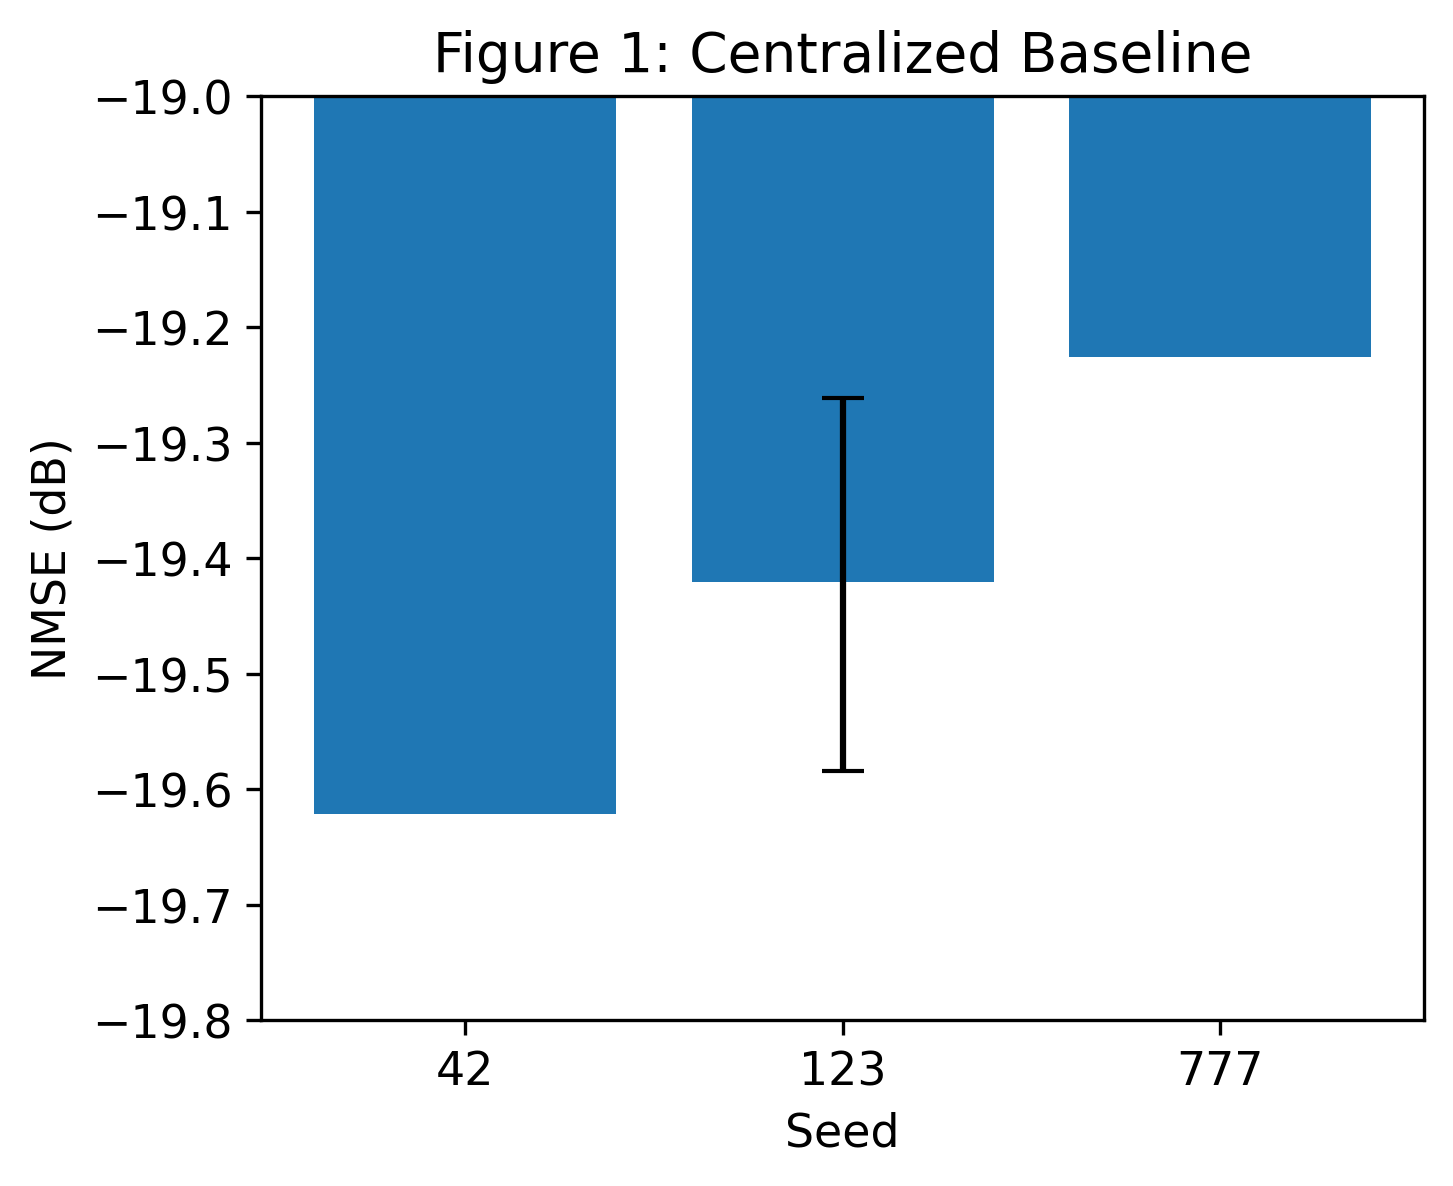
\includegraphics[width=0.75\columnwidth]{figures/figure1_centralized_baseline.png}
\caption{NMSE of the centralised CNN baseline across three random seeds
  at 10\,dB SNR.  The narrow inter-seed variance confirms the stability
  of the centralised training process, establishing a reliable reference
  for federated comparisons.}
\label{fig:f1}
\end{figure}

\subsection{Convergence Dynamics and Hyperparameter Sensitivity}
\label{ssec:hyper}

Fig.~\ref{fig:f2} shows that NMSE improves rapidly during the first
$\sim 20$ global rounds and then enters a diminishing-returns regime.
This is characteristic of FedAvg on IID data: after the initial
alignment phase, client updates become increasingly redundant, and
additional rounds yield marginal improvements.  Fig.~\ref{fig:f3}
demonstrates that increasing local epochs $E$ generally improves final
NMSE, since longer local training extracts more information per round.
However, the benefit saturates: very large $E$ can cause \emph{client
drift}, where local models diverge sufficiently from the global model
that their average no longer represents a consistent global optimum.

\begin{figure}[htbp]
\centering
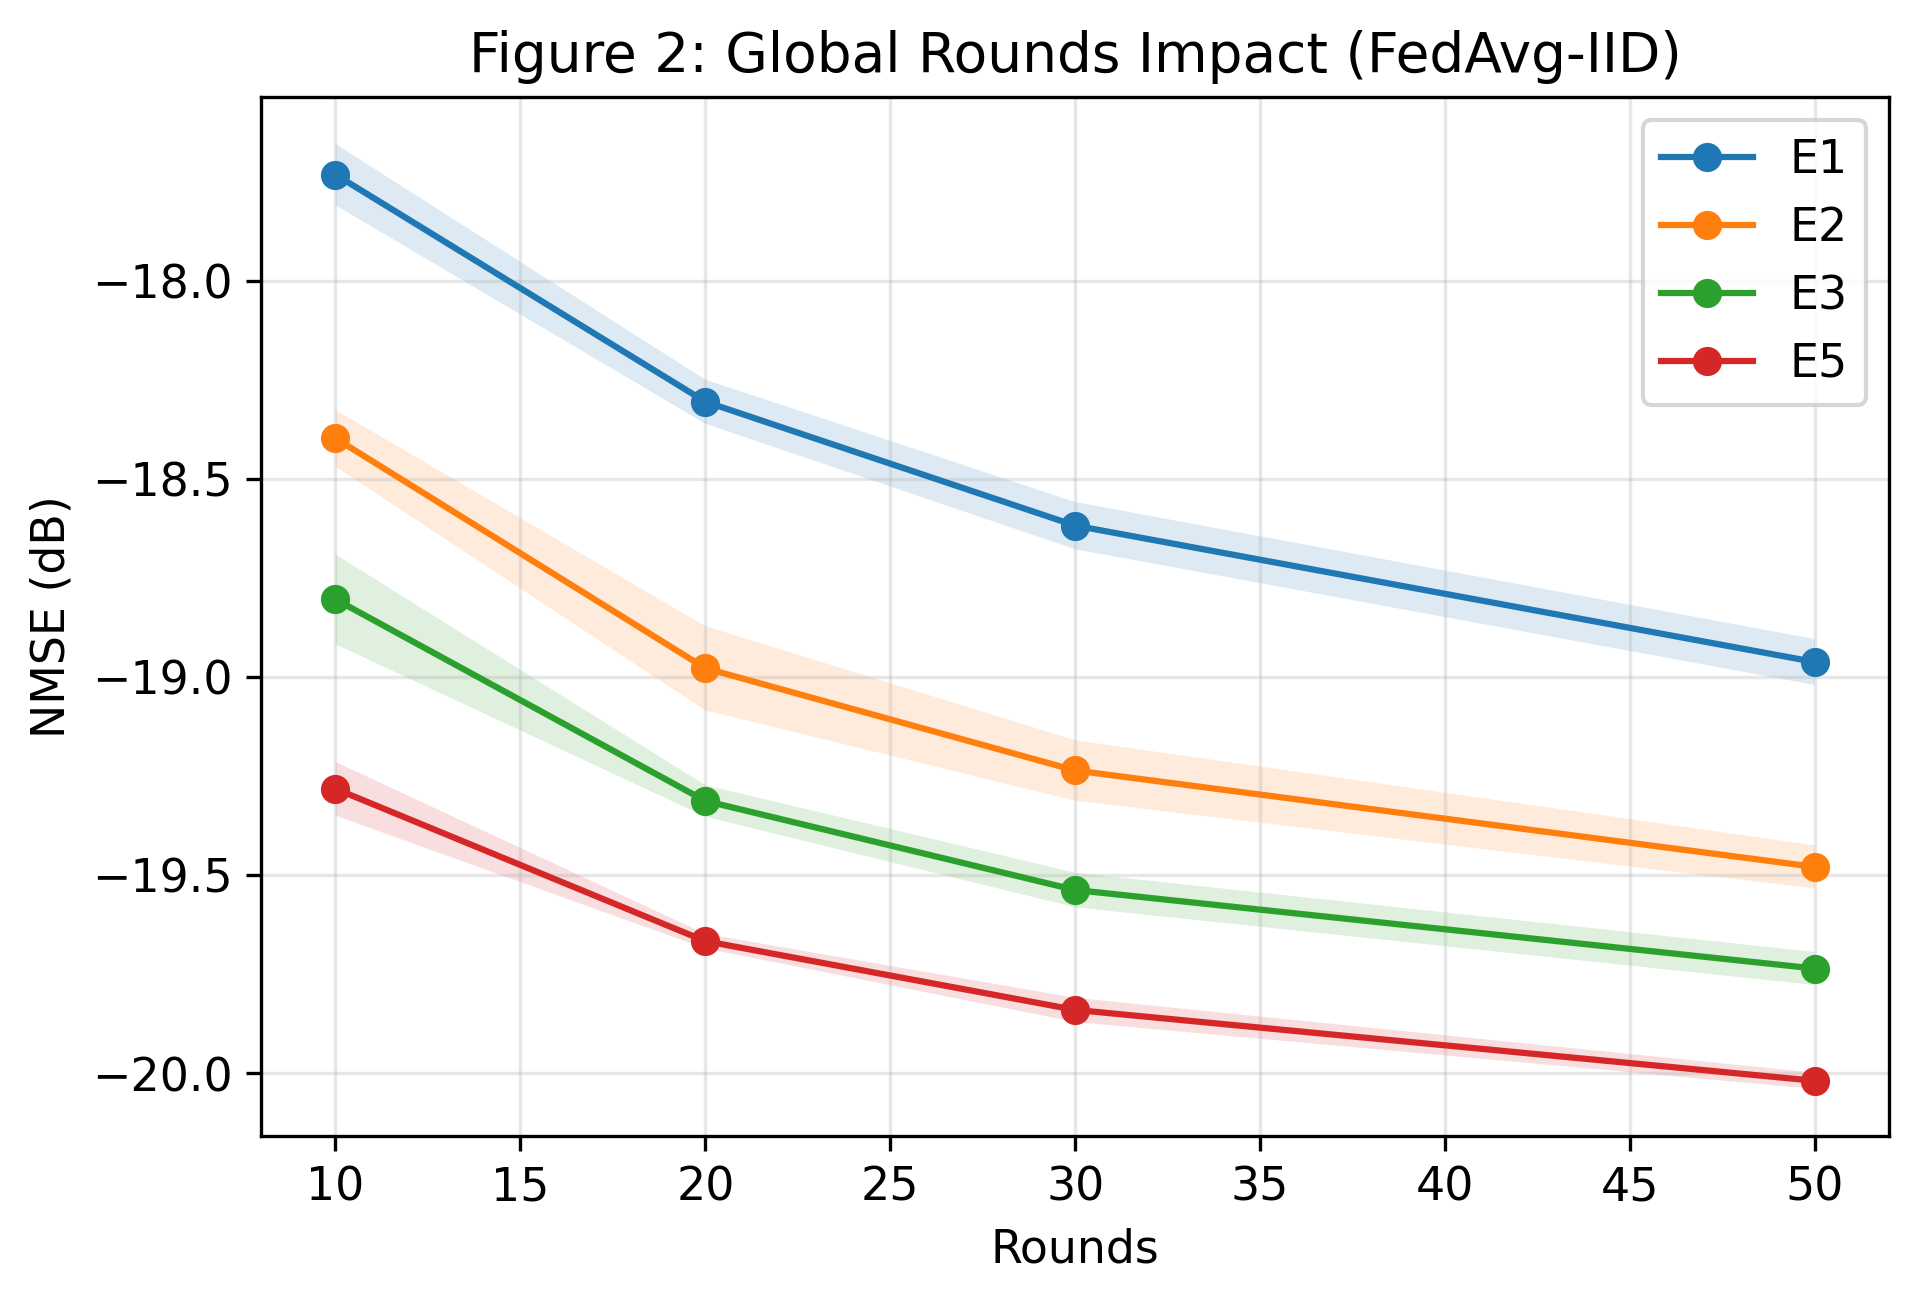
\includegraphics[width=0.65\columnwidth]{figures/figure2_rounds_impact_fedavg_iid.png}
\caption{Impact of global communication rounds on FedAvg-IID NMSE at
  $10$\,dB SNR.  Performance improves rapidly for $R \leq 20$
  and plateaus thereafter, indicating diminishing returns from
  additional communication rounds.}
\label{fig:f2}
\end{figure}

\begin{figure}[htbp]
\centering
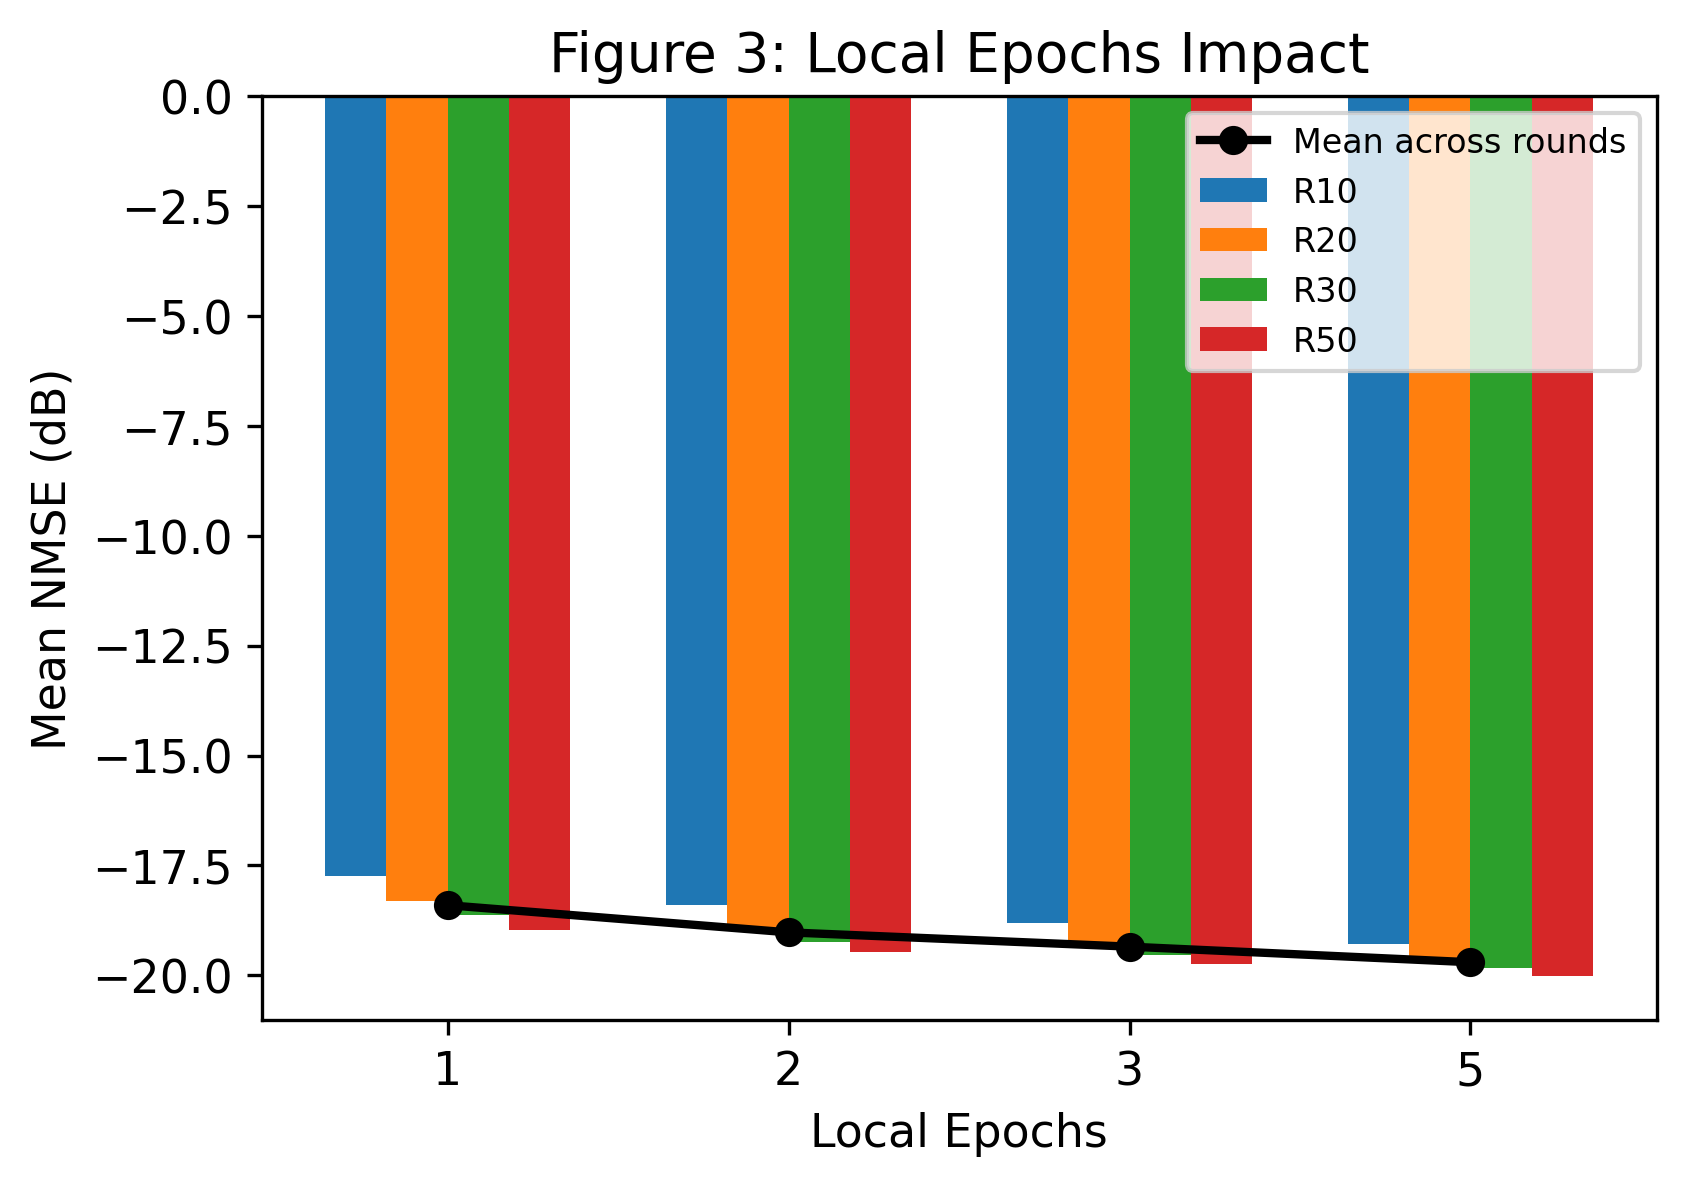
\includegraphics[width=0.65\columnwidth]{figures/figure3_local_epochs_impact.png}
\caption{Effect of local epoch count $E$ on FedAvg-IID final NMSE.
  Increasing local computation improves global convergence, though very
  large $E$ risks client-drift instability under heterogeneous data.}
\label{fig:f3}
\end{figure}

The round-by-round NMSE trajectories in Fig.~\ref{fig:f8} further
elucidate the convergence dynamics.  The IID curve exhibits a smooth,
monotonic descent, consistent with well-posed distributed optimisation.
By contrast, Non-IID curves display greater oscillation and converge to
a higher error floor, confirming that heterogeneity is an optimisation
process issue rather than merely an endpoint artefact.

\begin{figure}[htbp]
\centering
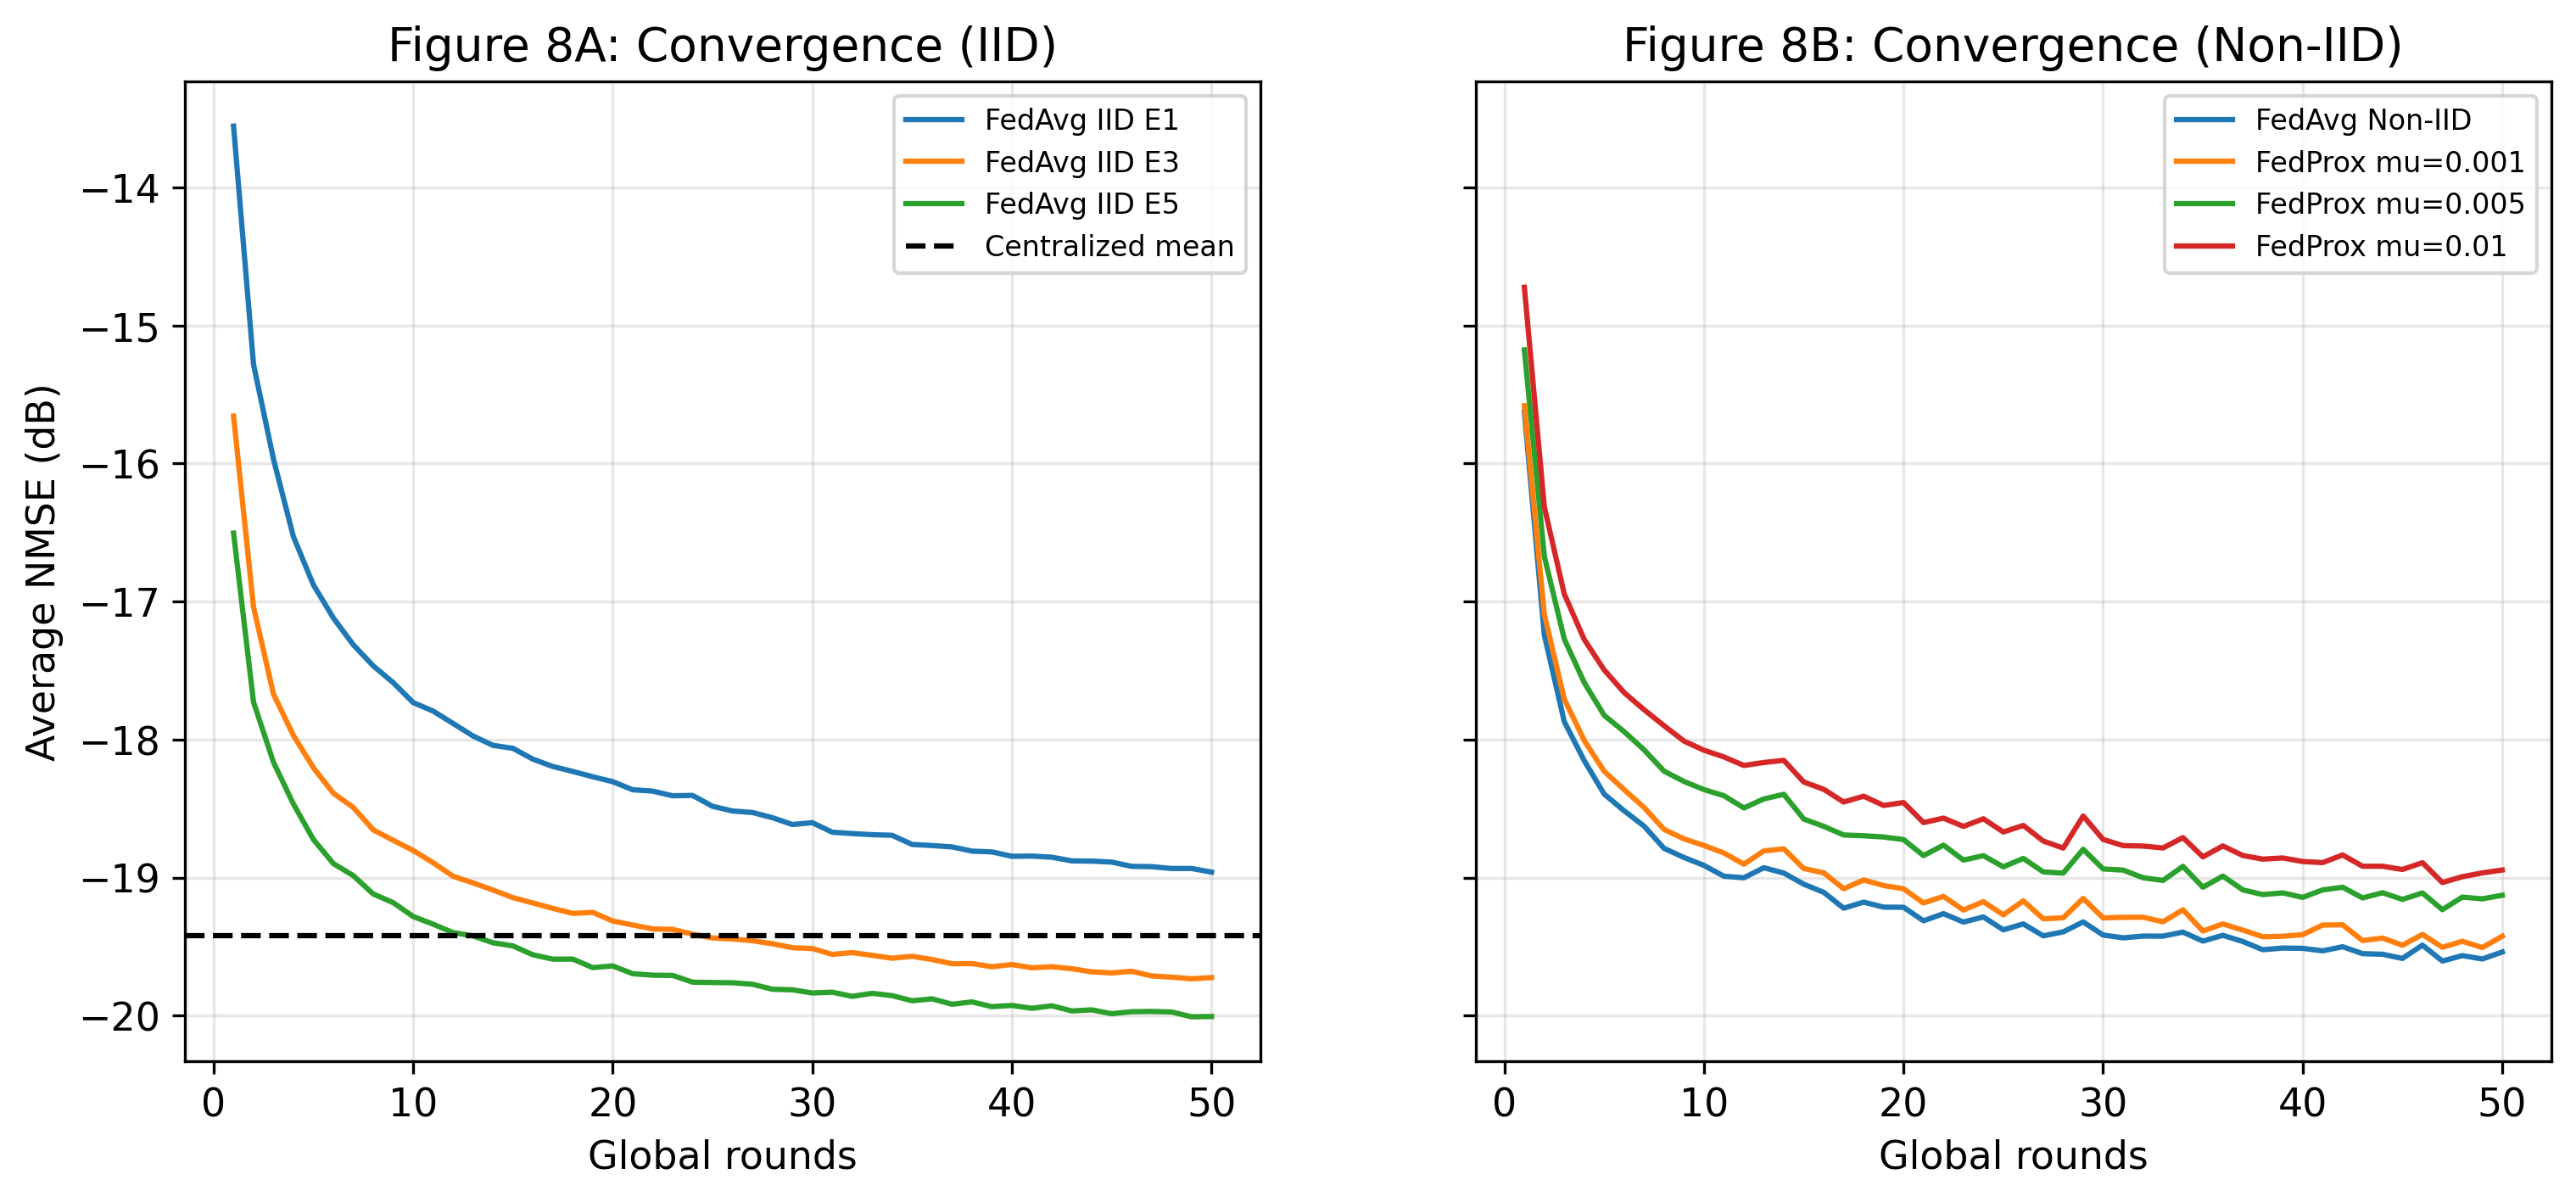
\includegraphics[width=0.75\columnwidth]{figures/figure8_convergence_curves.png}
\caption{Validation NMSE convergence trajectories across global rounds
  for representative IID and Non-IID FedAvg configurations.  The
  smoother IID descent and the oscillatory Non-IID behaviour visually
  confirm that data heterogeneity affects the optimisation trajectory,
  not only the final performance.}
\label{fig:f8}
\end{figure}

\subsection{IID vs.\ Non-IID and FedProx Behaviour}
\label{ssec:iid_noniid}

Fig.~\ref{fig:f4} visualises the NMSE distributions under IID and
Non-IID partitions.  The Non-IID distribution is shifted toward higher
error and exhibits greater spread, consistent with the statistical
summary in Table~\ref{tab:cnn_stats}.

\begin{figure}[htbp]
\centering
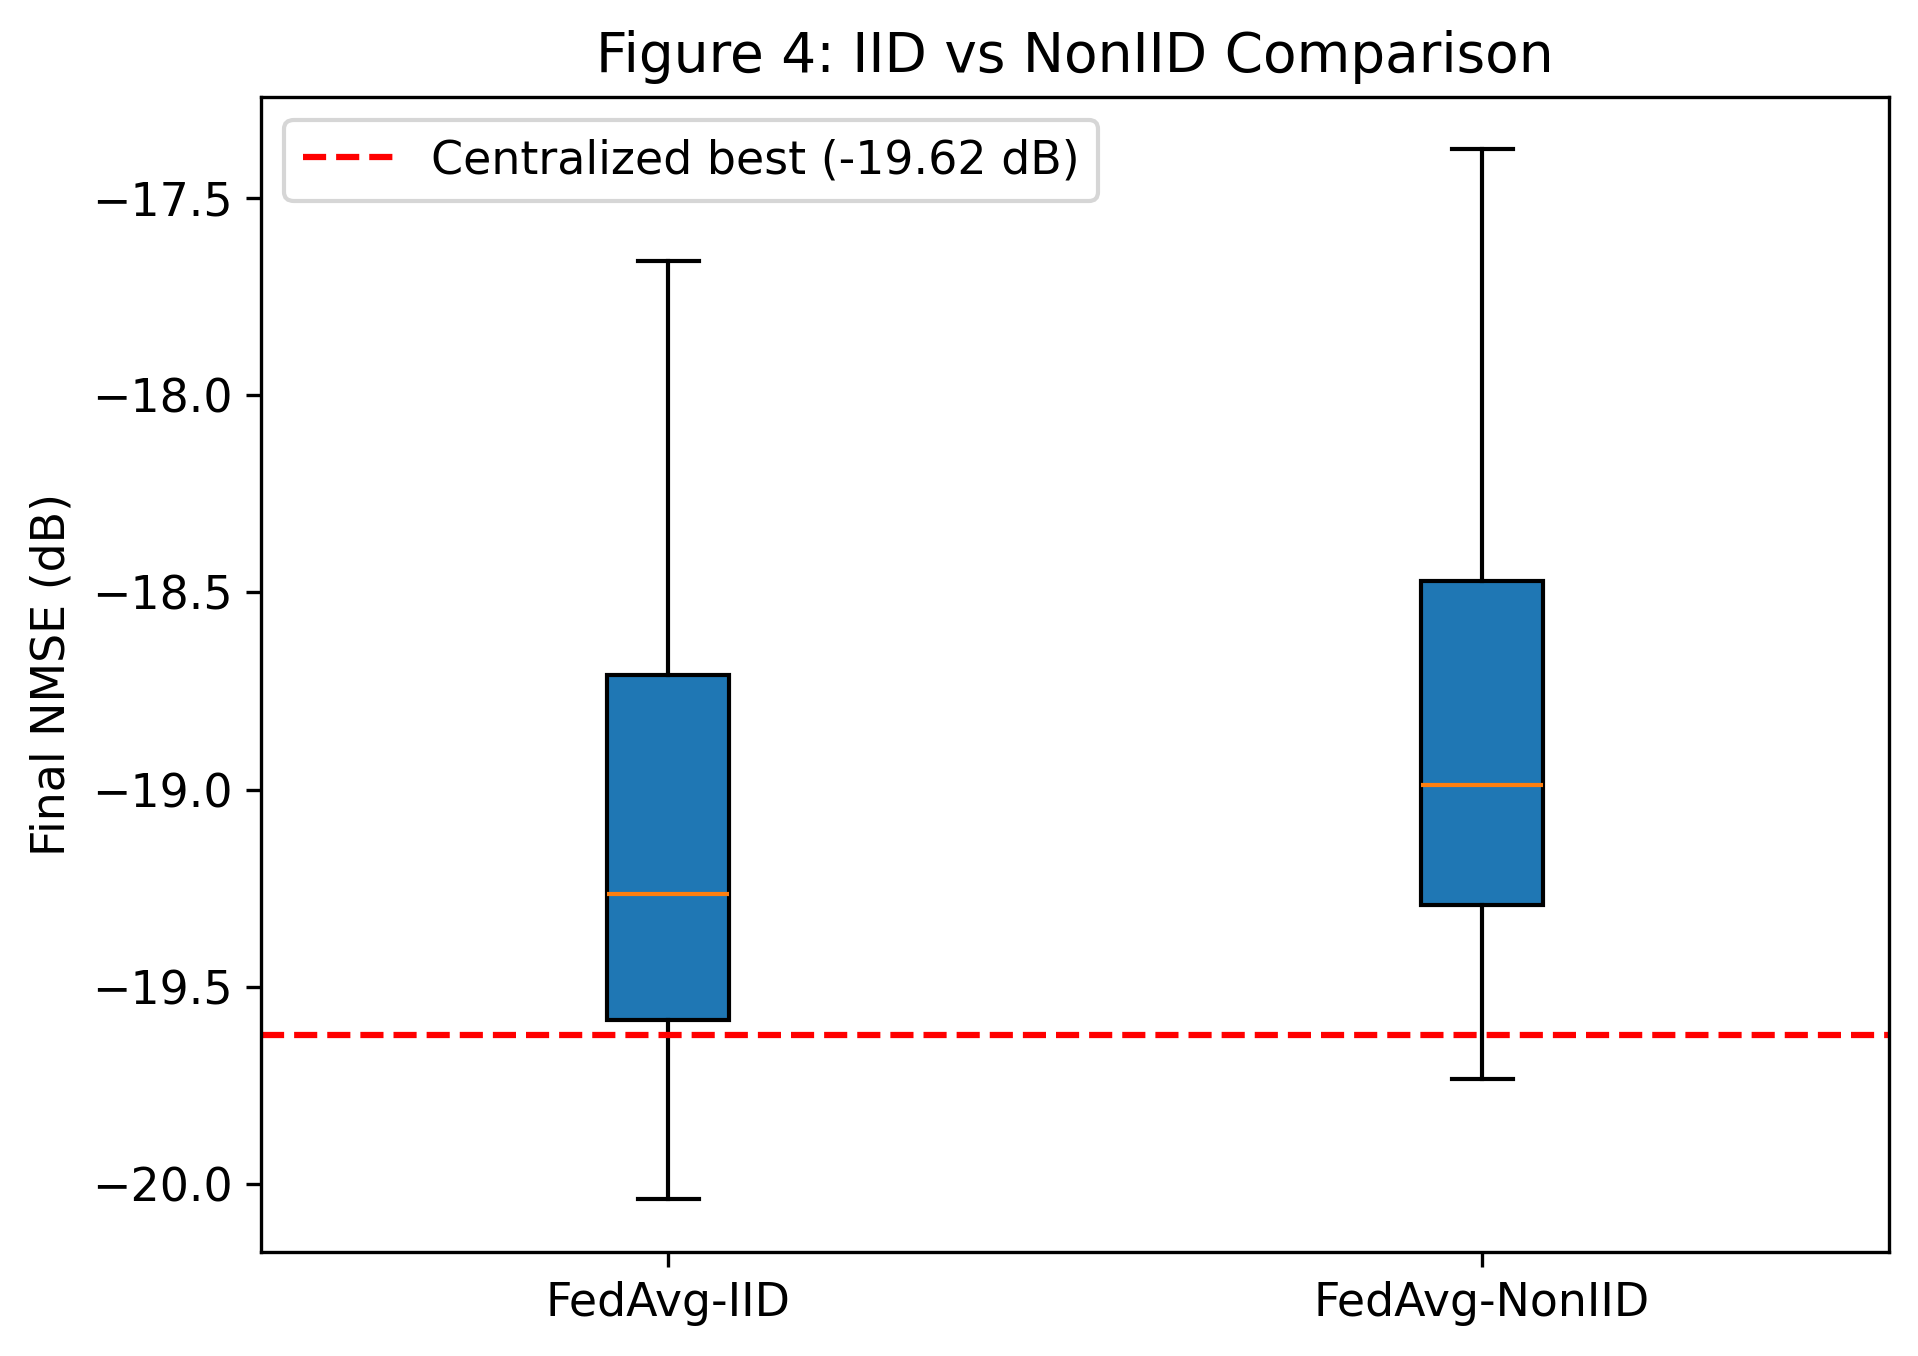
\includegraphics[width=0.75\columnwidth]{figures/figure4_iid_vs_noniid.png}
\caption{NMSE distributions under IID and Non-IID client partitioning
  at 10\,dB SNR.  Non-IID clients experience a shifted error
  distribution and higher variance relative to IID, quantifying the
  heterogeneity-induced degradation ($0.27$\,dB mean gap,
  Welch $p = 0.0289$).}
\label{fig:f4}
\end{figure}

FedProx adds the proximal term in Eq.~\eqref{eq:fedprox} to limit
client-drift, which we hypothesised would close the IID--Non-IID gap.
The results indicate, however, that FedProx-Non-IID further degrades
mean NMSE by $0.28$\,dB relative to FedAvg-Non-IID (Welch $p = 0.0044$).
Three complementary explanations account for this behaviour.

\textbf{Over-regularisation at limited local epochs.}  When $E$ is
small, the proximal penalty dominates before meaningful local fitting
occurs.  The ablation over $\mu \in \{0.001, 0.005, 0.01\}$ confirms
this: mean NMSE is best at $\mu = 0.001$ and the sensitivity span is
$0.42$\,dB, indicating that larger $\mu$ values over-constrain local
adaptation.

\textbf{Objective mismatch under structured heterogeneity.}  Under
norm-sorted Non-IID partitions, the disparity between client loss
surfaces is systematic rather than random.  In this regime, penalising
divergence from the global model prevents clients from learning
client-specific SNR statistics, which can actually \emph{improve}
global generalisation through implicit data augmentation.

\textbf{Regime-specific interaction.}  The local epoch sensitivity span
($0.97$\,dB) exceeds the $\mu$ span ($0.42$\,dB), suggesting that
communication budget (rounds $\times$ epochs) is the primary
hyperparameter in the tested regime, and that FedProx benefits may
emerge under more severe or random-label heterogeneity rather than
structured SNR skew.

Fig.~\ref{fig:f7} summarises best, worst, and mean statistics across
all tested algorithms, highlighting that variability---not just
mean-NMSE---should guide operating-point selection in practice.

\begin{figure}[htbp]
\centering
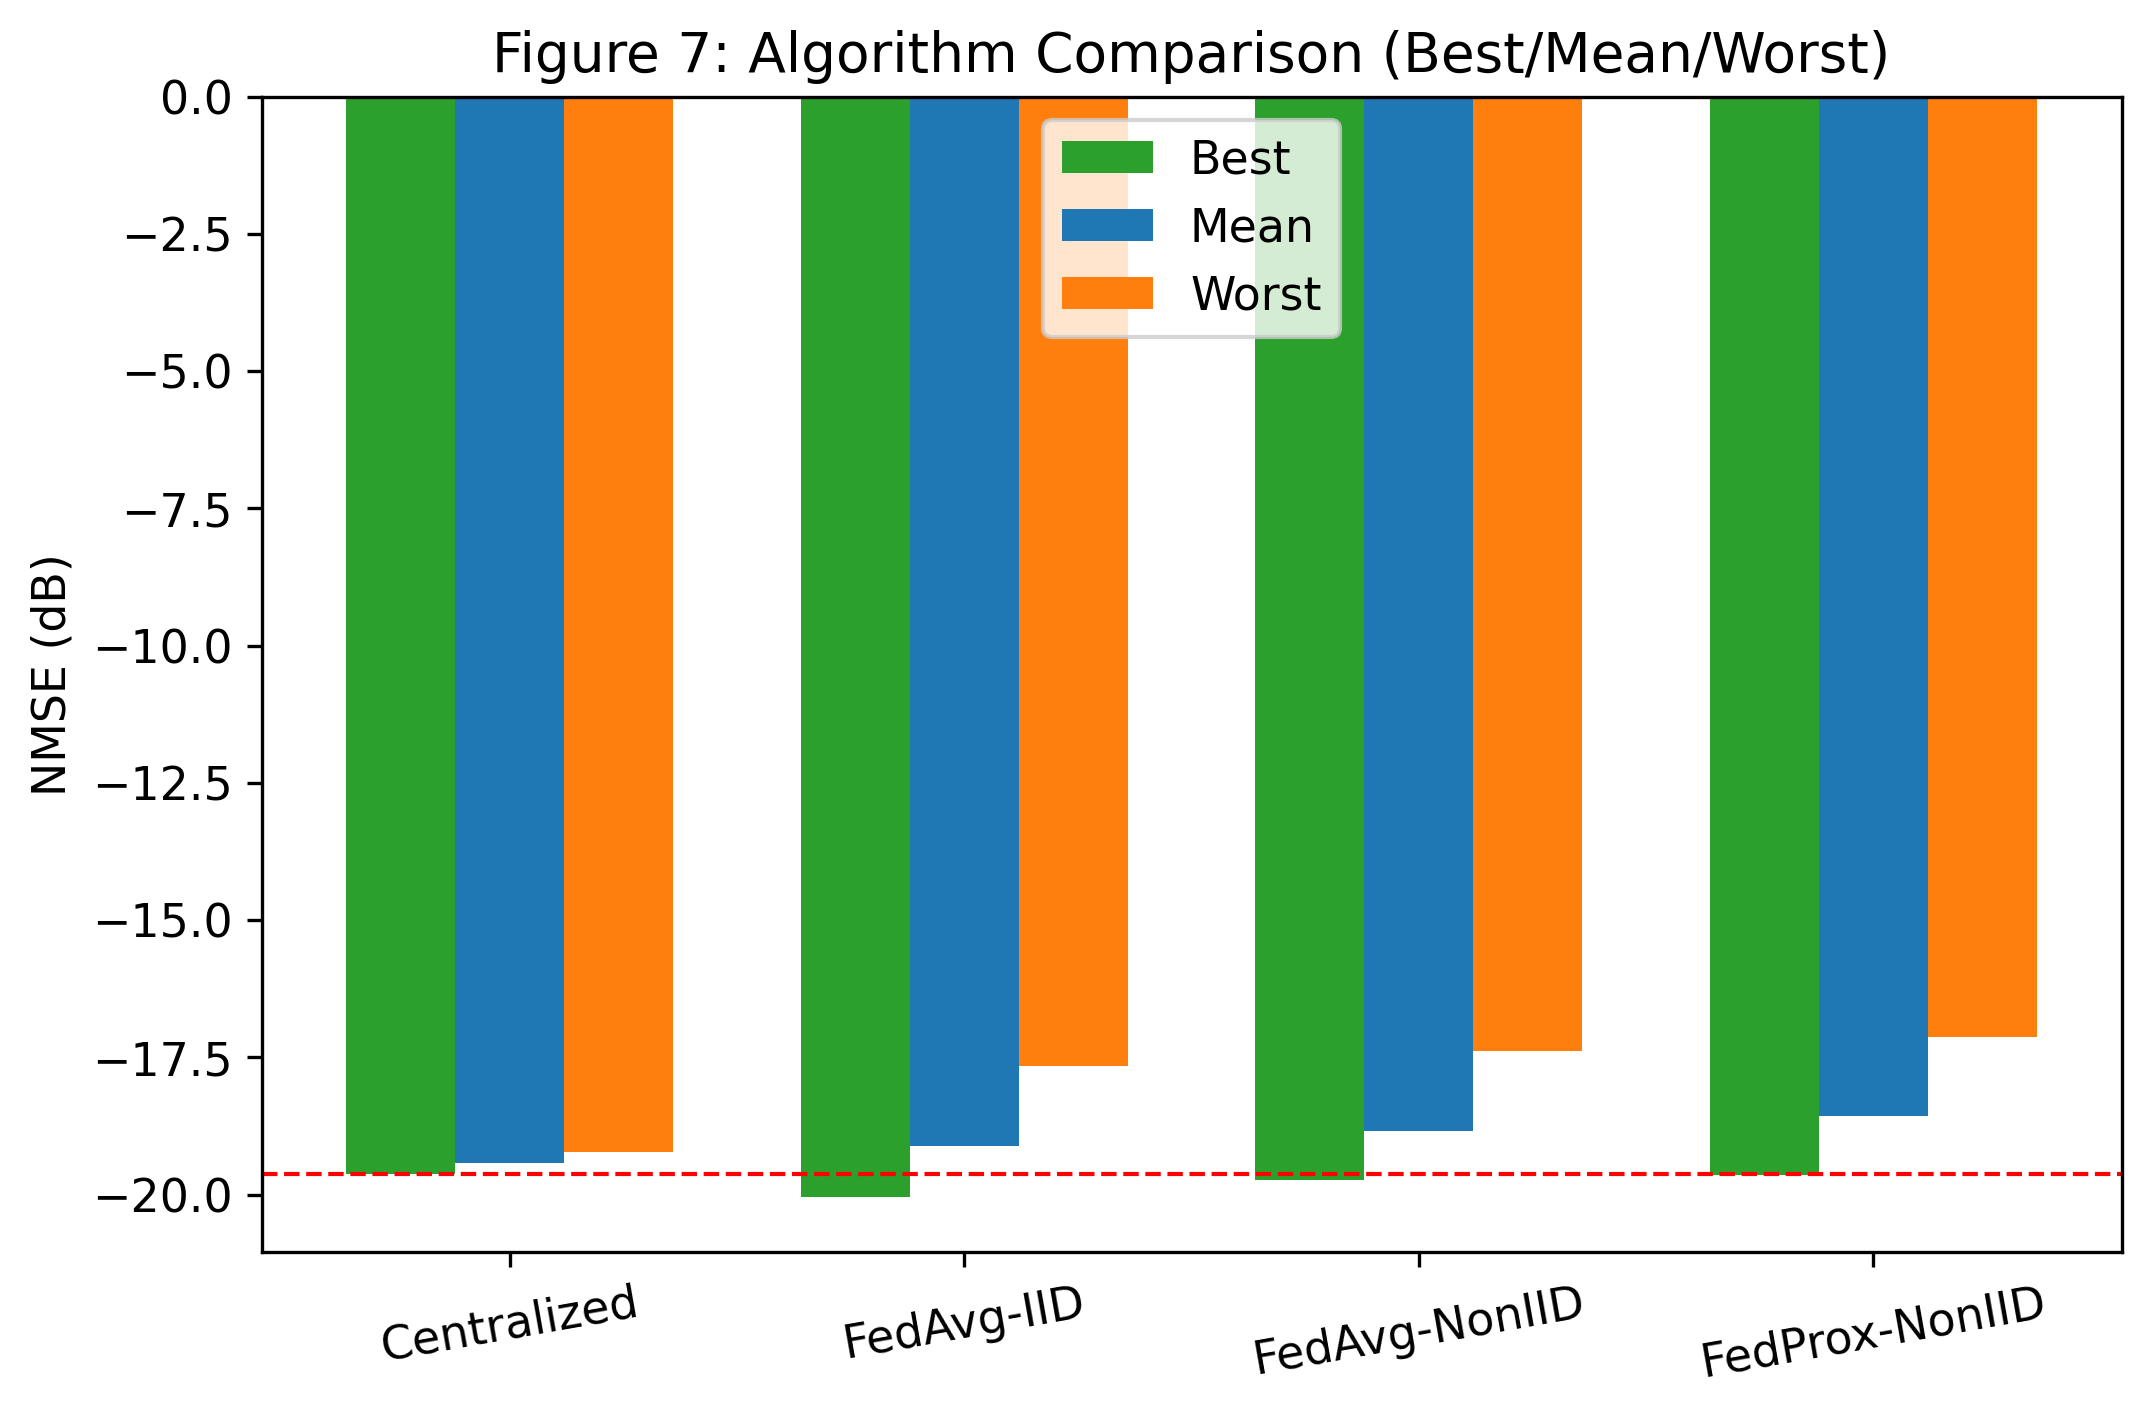
\includegraphics[width=0.75\columnwidth]{figures/figure7_algorithm_summary.png}
\caption{Best, worst, and mean NMSE statistics across all tested
  algorithms at 10\,dB SNR.  Wider bands in Non-IID settings indicate
  increased sensitivity to hyperparameters and seed variation,
  underscoring the need to report full distributional summaries rather
  than single best-run values.}
\label{fig:f7}
\end{figure}

\subsection{Cross-Architecture Consistency (ResUNet)}
\label{ssec:resunet}

Table~\ref{tab:resunet} and Fig.~\ref{fig:cross} confirm that the
heterogeneity penalty observed in the CNN persists across the heavier
ResUNet architecture.  FedAvg-IID achieves the lowest mean NMSE among
all federated settings ($-22.90$\,dB), outperforming the centralised
ResUNet baseline ($-22.12$\,dB), consistent with the CNN result.
FedAvg-Non-IID degrades by $+1.72$\,dB relative to FedAvg-IID for
ResUNet versus $+0.27$\,dB for the CNN, suggesting that deeper models
with larger per-client learning capacity amplify the effect of client
drift under structured heterogeneity.  The consistent trend across
architectures establishes heterogeneity as a data-distribution
phenomenon, not a model-specific artefact, motivating pipeline-level
rather than architecture-level mitigation strategies.

\begin{table}[htbp]
\caption{ResUNet add-on validation summary (5 seeds per setting,
  $10$\,dB SNR).  All NMSE values are in dB.}
\label{tab:resunet}
\centering
\begin{tabular}{lcccc}
\toprule
Setting & Runs & Mean (dB) & Std (dB) & Best (dB) \\
\midrule
Centralised      & 5 & $-22.12$ & $0.39$ & $-22.53$ \\
FedAvg-IID       & 5 & $-22.90$ & $0.13$ & $-23.04$ \\
FedAvg-Non-IID   & 5 & $-21.18$ & $0.34$ & $-21.62$ \\
FedProx-Non-IID  & 5 & $-20.47$ & $0.14$ & $-20.64$ \\
\bottomrule
\end{tabular}
\end{table}

\begin{figure}[htbp]
\centering
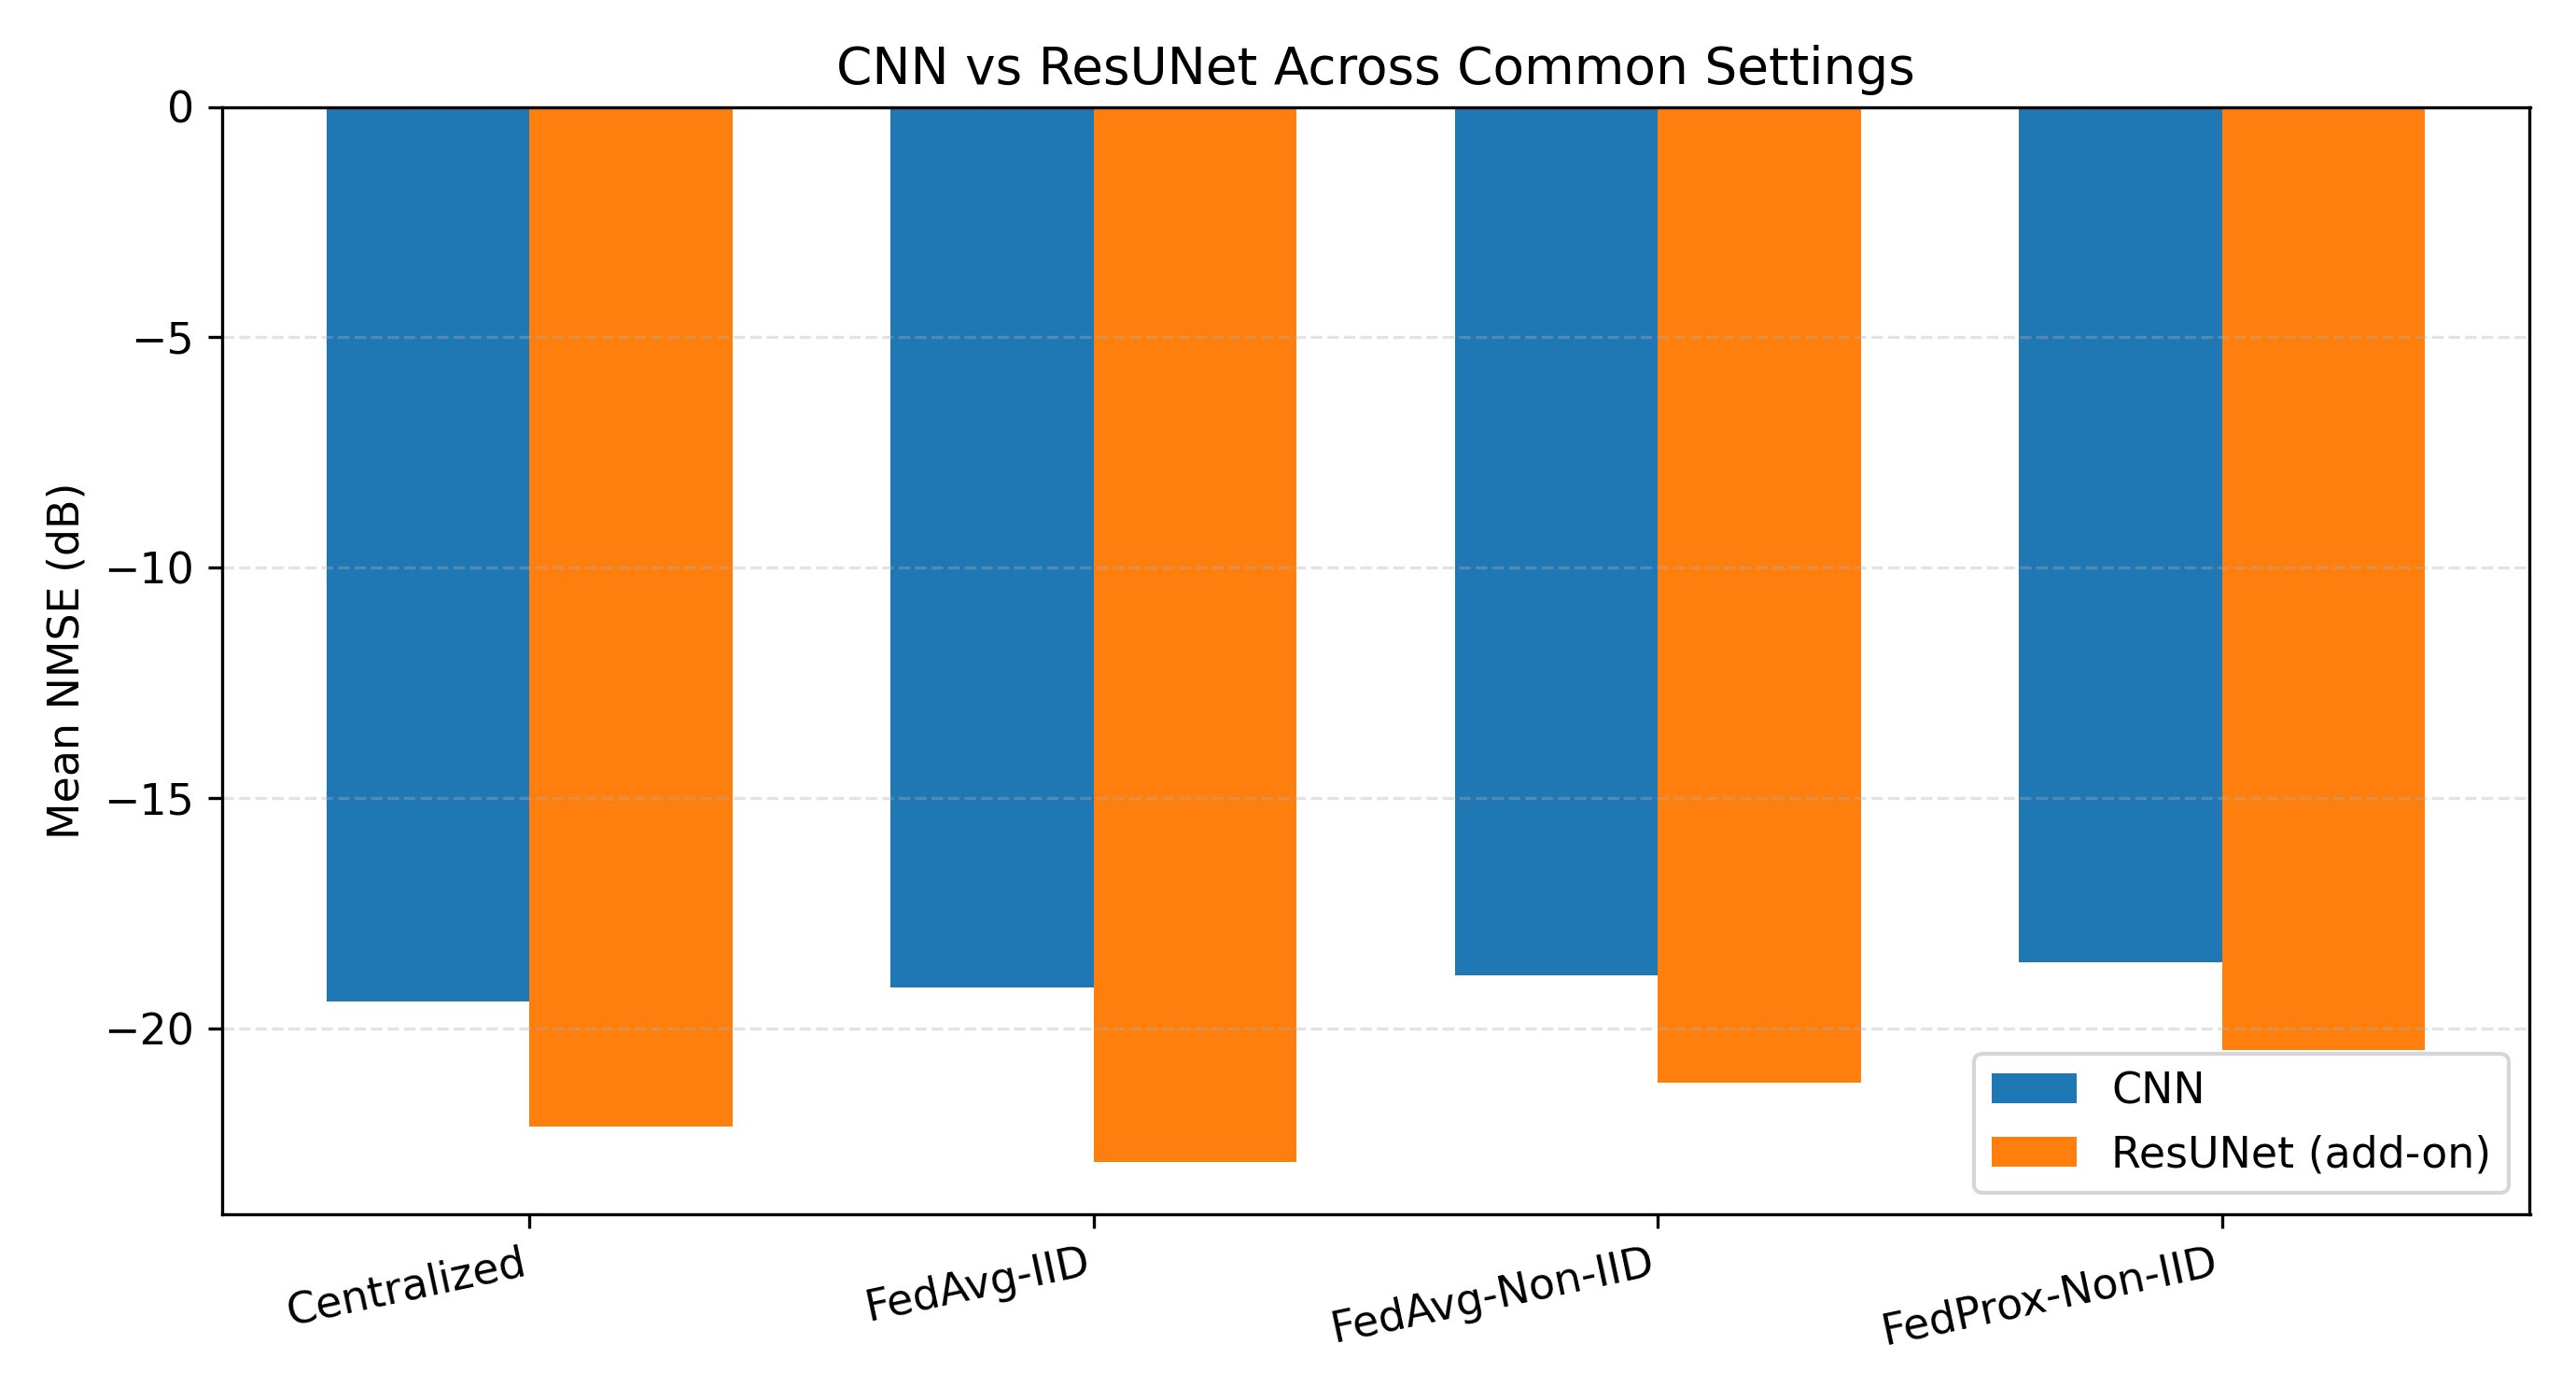
\includegraphics[width=0.75\columnwidth]{figures/resunet_addon_cnn_vs_resunet.png}
\caption{Comparative NMSE of CNN and ResUNet under aligned training
  settings.  Despite a $38\times$ difference in parameter count, both
  architectures exhibit the same trend ordering: FedAvg-IID~$<$
  Centralised~$<$ FedAvg-Non-IID~$<$ FedProx-Non-IID (where lower
  NMSE is better), confirming that the heterogeneity penalty is
  architecture-agnostic.}
\label{fig:cross}
\end{figure}

\subsection{Classical Baselines and Communication Analysis}
\label{ssec:classical}

Table~\ref{tab:classical} contextualises the deep learning results
against the classical estimators.  The CNN surpasses the LS estimator
by $9.42$\,dB because it leverages the nonlinear representational power
of convolutional filters to suppress channel-specific noise patterns
learned from training data---a capability entirely absent in the
unprocessed LS output $\hat{H}_\mathrm{LS} = \tilde{H}$.  The scalar
LMMSE provides a marginal $0.41$\,dB gain over LS by applying a
calibrated shrinkage factor, but it cannot model spatial correlations
across antenna elements or frequency-domain coherence, limiting its
performance at complex channel geometries.

The full-covariance MMSE achieves $-28.55$\,dB, substantially below
any deep model.  However, it requires the sample covariance matrix
$R_{HH}$ computed over the entire training set and an $O(d^3)$
inversion with $d = 8{,}192$, making it intractable in FL deployments
where each client holds only $\sim 960$ samples.  Deep models forgo
this covariance computation entirely, instead approximating the MMSE
nonlinearly through training, which explains their intermediate
performance.  Crucially, deep FL models remain viable precisely because
they do not require any centrally shared channel statistics to estimate
$R_{HH}$---the model weights themselves encode this knowledge
implicitly.

\begin{table}[htbp]
\caption{Classical estimator comparison and deep learning baselines at
  $10$\,dB SNR.  NMSE in dB; lower is better.}
\label{tab:classical}
\centering
\begin{tabular}{p{0.24\linewidth}p{0.14\linewidth}p{0.50\linewidth}}
\toprule
Method & NMSE (dB) & Notes \\
\midrule
LS             & $-10.00$ & $\hat{H} = \tilde{H}$; no noise suppression \\
Scalar LMMSE   & $-10.41$ & Train-calibrated scalar shrinkage \\
Full-Cov.\ MMSE & $-28.55$ & Wiener filter; $O(d^3)$ inversion required \\
\midrule
CNN (CL, mean) & $-19.42$ & $19{,}778$ params; no $R_{HH}$ required \\
ResUNet (CL, mean) & $-22.12$ & $763{,}234$ params; no $R_{HH}$ required \\
\bottomrule
\end{tabular}
\end{table}

\textbf{Communication cost model.}  Adopting FP32 precision, the uplink
payload per round per client is approximately $4P$ bytes, where $P$ is
the number of model parameters.  Total payload over all rounds is:
\begin{equation}
  \mathcal{C}_\mathrm{total} \approx 4PKR \quad \text{(bytes)},
  \label{eq:comm}
\end{equation}
with $K = 5$ clients.  For $R = 50$: the CNN requires $\approx 18.9$\,MB
while ResUNet requires $\approx 727.9$\,MB---a $38.6\times$ difference.

\textbf{Computational complexity.}  A single forward pass requires
$\sim\!160$\,MFLOPs for the CNN and $\sim\!2.5$\,GFLOPs for the
ResUNet---a $15.6\times$ ratio.  Table~\ref{tab:comm} summarises the
communication efficiency trade-off: the $R\!=\!50$, $E\!=\!5$
configuration delivers the highest NMSE ($-20.02$\,dB) but requires
$250$ communication events; the centralised baseline achieves
$-19.42$\,dB with zero federated communication events, illustrating
that the FL overhead is justified only when privacy preservation or
uplink bandwidth constraints preclude centralised training.

\begin{table}[htbp]
\caption{Communication cost snapshot for CNN-based FedAvg at 10\,dB
  SNR.  $R$ = global rounds, $E$ = local epochs,
  Comm.\ Events = $R \times K$.}
\label{tab:comm}
\centering
\begin{tabular}{lccc}
\toprule
Configuration & Comm.\ Events & NMSE (dB) & Efficiency \\
\midrule
FedAvg-IID ($R\!=\!10$, $E\!=\!1$) &  50 & $-17.73$ & Low \\
FedAvg-IID ($R\!=\!30$, $E\!=\!3$) & 150 & $-19.54$ & Medium \\
FedAvg-IID ($R\!=\!50$, $E\!=\!5$) & 250 & $-20.02$ & High \\
Centralised (20 epochs)             &   0 & $-19.42$ & Reference \\
\bottomrule
\end{tabular}
\end{table}

% ---------------------------------------------------------
\section{Conclusion}
\label{sec:conclusion}

We have presented a systematic and fully reproducible FL benchmark for
Massive MIMO channel estimation, encompassing CNN and ResUNet
architectures under FedAvg and FedProx across IID and Non-IID client
partitions.  The principal findings are as follows.  First, FedAvg-IID
achieves performance competitive with centralised training, with the
optimal configuration marginally exceeding the centralised NMSE,
demonstrating that privacy-preserving FL incurs negligible accuracy
cost under statistically homogeneous clients.  Second, Non-IID
heterogeneity introduces a consistent, statistically significant
degradation ($0.27$\,dB for CNN, $1.72$\,dB for ResUNet) attributable
to client drift and objective mismatch, and this effect is
architecture-agnostic.  Third, FedProx with the proximal coefficient
$\mu$ tuned conservatively does not consistently improve mean NMSE in
the tested regime; over-regularisation at limited local epochs prevents
clients from fully exploiting their local SNR-specific data
distributions.

Future work will extend the benchmark to the full SNR range
$(0\text{--}20)$\,dB, investigate personalised FL strategies tailored to
heterogeneous wireless clients, and explore pilot-based distributed
covariance estimation to further close the gap with the MMSE upper
bound.  Differentially private gradient aggregation represents a further
extension to strengthen privacy guarantees in the FL channel estimation
pipeline.

% ---------------------------------------------------------
\section*{Disclosure of Interests}

The authors have no competing interests to declare.

% ---------------------------------------------------------
\bibliographystyle{splncs04}
\bibliography{main}

\end{document}
